% Source: fixed 2015 Hunan science paper, printed page 955.
% Topological vector redraw; relative positions are schematic, not to scale.
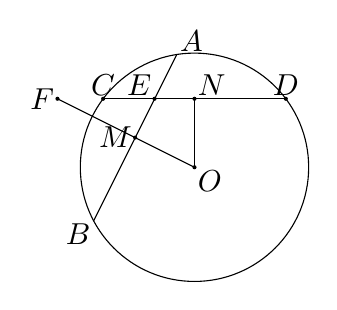
\begin{tikzpicture}[scale=1.45, every node/.style={font=\fontsize{10.5pt}{12.6pt}\selectfont, inner sep=1pt}]
  \coordinate (O) at (0,0);
  \coordinate (C) at (-.8,.6);
  \coordinate (D) at (.8,.6);
  \coordinate (N) at (0,.6);
  \coordinate (E) at (-.35,.6);
  \coordinate (M) at (-.52,.26);
  \coordinate (F) at (-1.20,.6);
  \draw (O) circle[radius=1];
  \draw (C)--(D);
  % Chord AB through E, perpendicular to OM; endpoints lie on the circle.
  \draw (-.883,-.468) -- (-.155,.988);
  \draw (F)--(O);
  \draw (O)--(N);
  \fill (O) circle[radius=.018] (C) circle[radius=.018] (D) circle[radius=.018]
        (E) circle[radius=.018] (M) circle[radius=.018] (N) circle[radius=.018] (F) circle[radius=.018];
  \node[above] at (C) {$C$};
  \node[above] at (D) {$D$};
  \node[above left] at (E) {$E$};
  \node[left] at (M) {$M$};
  \node[above right] at (N) {$N$};
  \node[left] at (F) {$F$};
  \node[below right] at (O) {$O$};
  \node[above right] at (-.155,.988) {$A$};
  \node[below left] at (-.883,-.468) {$B$};
\end{tikzpicture}
